\documentclass[serif, aspectratio=169]{beamer}
%\documentclass[serif]{beamer}  % for 4:3 ratio

\usepackage[T1]{fontenc} 
\usepackage[utf8]{inputenc}
\usepackage{fourier} % see "http://faq.ktug.org/wiki/uploads/MathFonts.pdf" for other options
\usepackage{hyperref}
\usepackage{latexsym,amsmath,xcolor,multicol,booktabs,calligra}
\usepackage{graphicx,pstricks,listings,stackengine}
\usepackage{lipsum}
\usepackage{../HKUSTstyle}

%imports customs%
\usepackage{caption}    % for subfigures
\usepackage{subcaption} % for subfigures
\usepackage{ragged2e}
\usepackage{booktabs,makecell}
\usepackage{colortbl}
\usepackage{multirow}
\usepackage{cite}
\usepackage{tcolorbox}
\usepackage[sort,authoryear]{natbib}

\author{Julien Bezançon}

\title{Python Programmation}
\subtitle{CM 2~: Data Structures}

\institute{julien.bezancon@univ-lorraine.fr / \url{https://julienbez.github.io}}

\date{}

% defs
\def\cmd#1{\texttt{\color{red}\footnotesize $\backslash$#1}}
\def\env#1{\texttt{\color{blue}\footnotesize #1}}

% set colors
\definecolor{hkustyellow}{RGB}{167, 131, 55}
\definecolor{hkustblue}{RGB}{0, 56, 116}
\definecolor{hkustred}{RGB}{209, 51, 59}

% easy colors
\newcommand{\tred}[1]{\textcolor{red!50}{#1}}
\newcommand{\tgreen}[1]{\textcolor{green}{#1}}
\newcommand{\tyellow}[1]{\textcolor{yellow}{#1}}
\newcommand{\tpurple}[1]{\textcolor{purple!50}{#1}}

% CLI environment
\newenvironment{CLI} % Command Line Interface
    {
    \noindent
    \ttfamily 
    \footnotesize
    \begin{tcolorbox}[colback=gray!150,colframe=black]
    \color{white}
    \begin{tabular}{p{4.5cm}p{7.5cm}}
    }
    { 
    \end{tabular}
    \end{tcolorbox}
    }

% Exercice environment
\newenvironment{exoframe}
    {
    \setbeamercolor{background canvas}{bg=hkustblue}
    \renewcommand\thefootnote{\textcolor{white}{\arabic{footnote}}}
    \color{white}
    \setbeamercolor{structure}{fg=white}
    \begin{frame}
    }
    {
    \end{frame}
    }

\lstset{
    basicstyle=\ttfamily\small,
    keywordstyle=\bfseries\color{deepblue},
    emphstyle=\ttfamily\color{deepred},    % Custom highlighting style
    stringstyle=\color{deepgreen},
    numbers=left,
    numberstyle=\small\color{halfgray},
    rulesepcolor=\color{red!20!green!20!blue!20},
    frame=shadowbox,
}

\begin{document} %  --- --- --- --- --- --- --- --- --- --- --- --- 

\begin{frame}[noframenumbering,plain]
    \titlepage
    \vspace*{-0.6cm}
    \begin{figure}[htpb]
        \begin{center}
            \hspace{0.3cm}
            
\includegraphics[width=0.7\columnwidth]{../../../IMAGES/loria_idmc.png}
        \end{center}
    \end{figure}
\end{frame}

% \begin{frame}    
%     \tableofcontents[sectionstyle=show,
%     subsectionstyle=show/shaded/hide,
%     subsubsectionstyle=show/shaded/hide]
% \end{frame}

\section{Before we start...}

\begin{exoframe}
    \begin{center}
        \Large
        What did you learn during last lecture ? \\
        Any questions ?
    \end{center}
\end{exoframe}

\begin{frame}{Last Lecture Doggy bag}
    \begin{minipage}{0.45\columnwidth}
        \begin{block}{Python Basics}
            \begin{itemize}
                \item Variables and types
                \item Operators
                \item Console input/output
                \item File manipulation
            \end{itemize}
        \end{block}
        \begin{block}{Control Flow}
            \begin{itemize}
                \item Statements
                \item Loops
                % \item Range
            \end{itemize}
        \end{block}
    \end{minipage}
    \hfill
    \begin{minipage}{0.45\columnwidth}
        \begin{figure}
            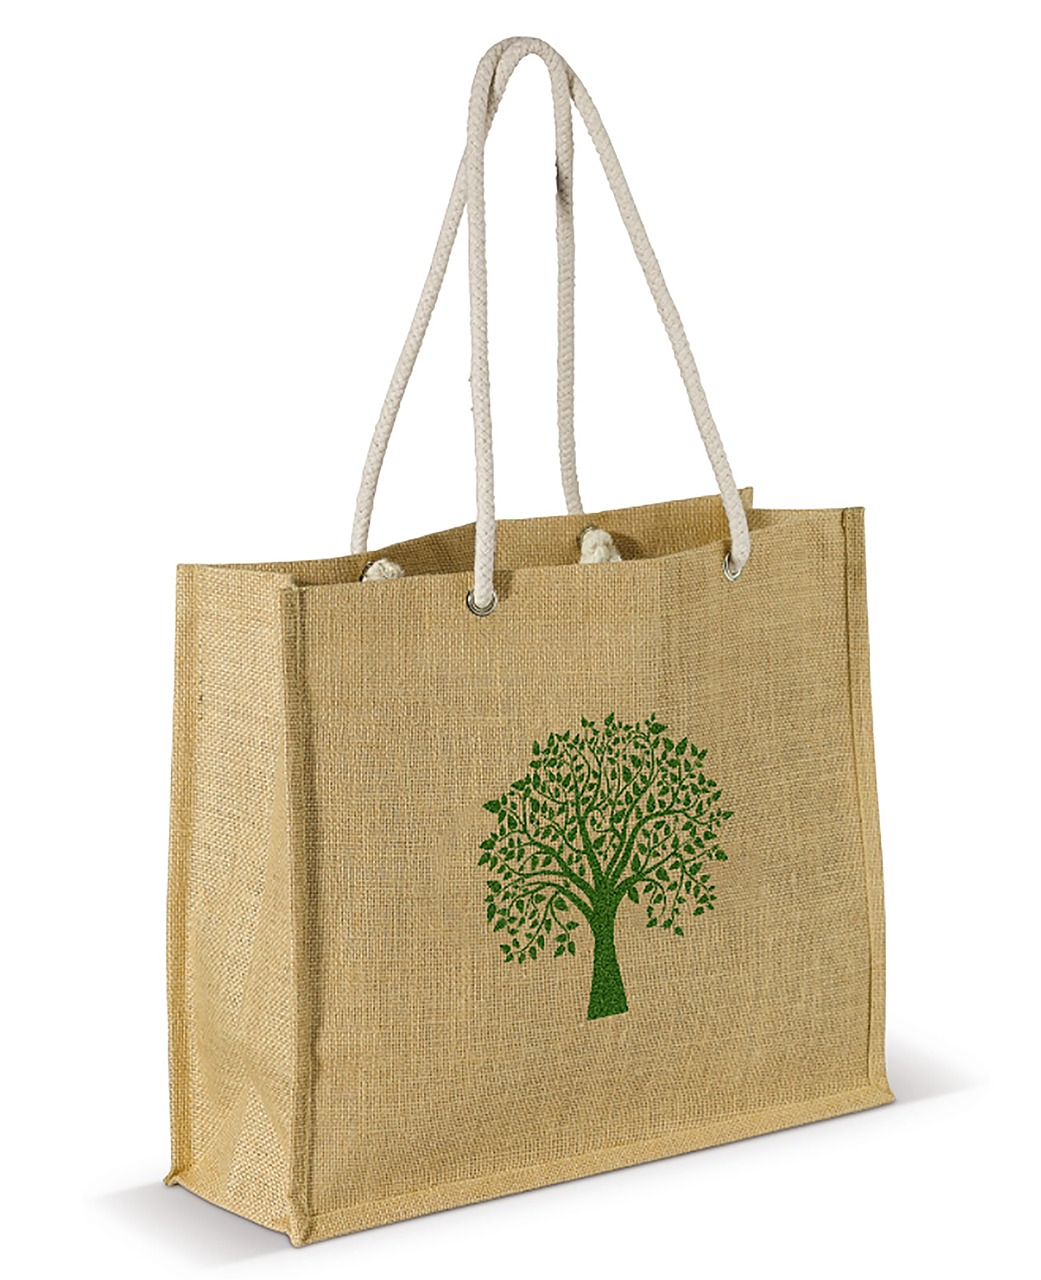
\includegraphics[width=0.9\columnwidth]{../../../FIGURES/divers/doggybag.jpg}
        \end{figure}
    \end{minipage}
\end{frame}

\section{Lists}

\begin{frame}{Lists}
     \begin{block}{Lists are object which contain other objects}
        \vspace{2pt}
        \begin{CLI}
            \tgreen{\# Brackets delimit a list} & \\
            \multicolumn{2}{l}{\tgreen{\# Commas separate its elements}} \\
            & \\
            a\_list = [1,2,3] & \\
            b\_list = ['a','b','c','d'] & \\
            \pause
            & \\
            \multicolumn{2}{l}{\tgreen{\# A list can contain elements of different types}} \\
            \multicolumn{2}{l}{mixed\_list = [4,5,"seconds"]} \\
            \pause
            & \\
            \multicolumn{2}{l}{\tgreen{\# Elements can be added to the end of a list}} \\
            empty\_list = [] & \tgreen{\# List without any element} \\
            empty\_list.append(7) & \tgreen{\# => empty\_list == [7]} \\
            empty\_list.append("kebab") & \tgreen{\# => empty\_list == [7,"kebab"]} \\
        \end{CLI}
     \end{block}
\end{frame}

\begin{frame}{List Indexing and Slicing}
    \begin{block}{Same as string indexing and slicing}
        \vspace{2pt}
        \begin{CLI}
            \multicolumn{2}{l}{letters = ['a', 'b', 'c', 'd']} \\
            numbers = [2, 3, 5, 7, 11] & \\
            \pause
            & \\
            \multicolumn{2}{l}{\tgreen{\# Access elements at a particular index}} \\
            numbers[0] & \tgreen{\# => 2} \\
            numbers[-1] & \tgreen{\# => 11}  \\
            \pause
            & \\
            \multicolumn{2}{l}{\tgreen{\# The same rules apply of slicing}} \\
            letters[:3] & \tgreen{\# => ['a', 'b', 'c']} \\
            numbers[1:-1] & \tgreen{\# => [3, 5, 7]} \\
        \end{CLI}
    \end{block}
\end{frame}

\begin{frame}{Nested lists}
    \begin{block}{Lists can even contain other lists !}
        \vspace{2pt}
        \begin{CLI}
            \multicolumn{2}{l}{letters = ['a', 'b', 'c', 'd']} \\
            numbers = [2, 3, 5, 7, 11] & \\
            \pause
            & \\
            combo = [letters, numbers] & \tgreen{\# => [['a', 'b', 'c', 'd'], [2, 3, 5, 7, 11]]} \\
            combo[0] & \tgreen{\# => ['a', 'b', 'c', 'd']} \\
            combo[0][1] & \tgreen{\# => 'b'} \\
            combo[1][2:] & \tgreen{\# => [5, 7, 11]} \\
        \end{CLI}
    \end{block}
\end{frame}

\begin{frame}{List Methods}
    \begin{CLI}
        \multicolumn{2}{l}{\tgreen{\# Extend list by appending elements from the iterable}} \\
        my\_list.extend(another\_list) & \\
         & \\
        \multicolumn{2}{l}{\tgreen{\# Insert object before index}} \\
        \multicolumn{2}{l}{my\_list.insert(index, object)} \\
         & \\
        \multicolumn{2}{l}{\tgreen{\# Remove first occurrence of value, or raise ValueError}} \\
        my\_list.remove(value) & \\
         & \\
        \multicolumn{2}{l}{\tgreen{\# Remove all items}} \\
        my\_list.clear() & \\
    \end{CLI}
\end{frame}


\begin{frame}{List Methods}
    \begin{CLI}
        \multicolumn{2}{l}{\tgreen{\# Return number of occurrences of value}} \\
        my\_list.count(value) & \\
        & \\
        \multicolumn{2}{l}{\tgreen{\# Return first index of value, or raise ValueError}} \\
        \multicolumn{2}{l}{my\_list.index(value, [start, [stop]])} \\
        & \\
        \multicolumn{2}{l}{\tgreen{\# Remove, return item at index (def. last) or IndexError}} \\
        my\_list.pop([index]) & \\
        & \\
        \multicolumn{2}{l}{\tgreen{\# Stable sort *in place*}} \\
        \multicolumn{2}{l}{my\_list.sort(key=None, reverse=False)} \\
        & \\
        \multicolumn{2}{l}{\tgreen{\# Reverse *in place*.}} \\
        my\_list.reverse() & \\
    \end{CLI}
\end{frame}

\begin{frame}{General Queries}
    \begin{block}{some useful queries in Python}
        \vspace{2pt}
        \begin{CLI}
            \tgreen{\# Length (len)} & \\
            len([]) & \tgreen{\# => 0} \\
            len("python") & \tgreen{\# => 6} \\
            len([4, 5, "seconds"]) & \tgreen{\# => 3} \\
            \pause
            & \\
            \tgreen{\# Membership (in)} & \\
            0 in [] & \tgreen{\# => False} \\
            'y' in "python" & \tgreen{\# => True} \\
            "sec" in [4, 5, "seconds"] & \tgreen{\# => False} \\
            & \\
            max([1,2,3,4,5]) & \tgreen{\# => 5} \\
            min([1,2,3,4,5]) & \tgreen{\# => 1} \\
        \end{CLI}        
    \end{block}
\end{frame}

\begin{exoframe}
    \begin{block}{}
        \begin{itemize} \color{white}
            \item[1.] Create the following list: [1,2,2,3,3,3,4,4,4,4]
            \item[2.] Count the number of occurrence of each value in this list
            \vspace{10pt}
            \item[3.] Add the number 10.000 at the end of this list
            \item[4.] Add the number 0 at the begining of this list
            \vspace{10pt}
            \item[5.] Remove all values which are multiple of two
            \item[6.] Print the total number of elements in this list    
        \end{itemize}
    \end{block}
\end{exoframe}

\section{Dictionaries}

\begin{frame}{Dictionaries}
    \begin{CLI}
        empty\_dict = \{\} & \\
        \multicolumn{2}{l}{a\_dict = \{"one":1, "two":2, "toto":3\}} \\
        & \\
        print(empty\_dict) & \\
        % \tgreen{\# => \{\}} & \\
        & \\
        print(a\_dict) & \\
        % \multicolumn{2}{l}{\tgreen{\# => \{"one":1, "two":2, "toto":3\}}} \\
    \end{CLI}
    \begin{block}{}
        \begin{itemize}
            \item Dictionaries store data in "key":"value" pairs 
            \item As of Python 3.7, dictionaries are ordered
            \item They do not allow duplicates !
        \end{itemize}
    \end{block}
\end{frame}

\begin{frame}{Dictionary Indexes}
    \begin{CLI}
        \multicolumn{2}{l}{a\_dict = \{"one": 1, "two": 2, "three": 3\}} \\
        & \\
        \tgreen{\# Get} & \\
        d["one"] & \\%\tgreen{\# => 1} \\
        d["five"] & \\%\tgreen{\# raises KeyError} \\
        & \\
        \tgreen{\# Set} & \\
        d["two"] = 22 & \tgreen{\# Modify an existing key} \\
        d["four"] = 4 & \tgreen{\# Add a new key} \\
        & \\
        \multicolumn{2}{l}{\tgreen{\# Advanced way of adding an element}} \\
        a\_dict.setdefault("five",5) & \\
    \end{CLI}
\end{frame}

\begin{frame}{get Method}
    \begin{CLI}
        \multicolumn{2}{l}{d = \{"CS":[106, 107, 110], "MATH": [51, 113]\}} \\
        d["COMPSCI"] & \\%\tgreen{\# raises KeyError} \\
        & \\
        \multicolumn{2}{l}{\tgreen{\# Use get() method to avoid the KeyError}} \\
        d.get("CS") & \\%\tgreen{\# => [106, 107, 110]} \\
        d.get("PHIL") & \\%\tgreen{\# => None (not a KeyError!)} \\
        & \\
        \multicolumn{2}{l}{english\_classes = d.get("ENGLISH", [])} \\
        \multicolumn{2}{l}{num\_english = len(english\_classes)} \\
        & \\
        \multicolumn{2}{l}{math\_classes = d.get("MATH",[])} \\
        \multicolumn{2}{l}{num\_math = len(math\_classes)} \\
    \end{CLI}
\end{frame}

\begin{frame}{Delete Method}
    \begin{CLI}
        \multicolumn{2}{l}{d = \{"one": 1, "two": 2, "three": 3\}} \\
        & \\
        del d["one"] & \tgreen{\# Raises KeyError if invalid key} \\
        & \\
        \multicolumn{2}{l}{\tgreen{\# Remove and return d['three'] or default value if not in the map}} \\
        d.pop("three", default) & \\
        & \\
        \multicolumn{2}{l}{\tgreen{\# Remove and return an arbitrary (key, value) pair}} \\
        %\multicolumn{2}{l}{\tgreen{\# Useful for destructive iteration}} \\
        d.popitem() & \tgreen{\# => ("two", 2)} \\
    \end{CLI}
\end{frame}

\begin{frame}{Dictionary View}
    \begin{CLI}
        \multicolumn{2}{l}{d = \{"one": 1, "two": 2, "three": 3\}} \\
        & \\
        d.keys() & \\
        d.values() & \\
        d.items() & \\
        & \\
        len(d.keys()) & \\%\tgreen{\# => 3} \\
        & \\
        \multicolumn{2}{l}{\tyellow{for} key,value \tyellow{in} d.items():} \\
        ~~print(key,value) & \\
        & \\
        \multicolumn{2}{l}{keys\_list = list(d.keys())} \\
    \end{CLI}
\end{frame}

\begin{exoframe}
    \begin{block}{}
        \begin{itemize} \color{white}
            \item[1.] Create a dictionary with 5 pairs of key:value in it
            \item[2.] Add the following pair: "answer":42
            \vspace{10pt}
            \item[3.] Change all values of this dictionary to 42
            \item[4.] Remove the key "answer" from this dictionary
            \vspace{10pt}
            \item[5.] Print every keys from this dictionary
            \item[6.] Print every values from this dictionary    
        \end{itemize}
    \end{block}
\end{exoframe}

\section{Tuples}

\begin{frame}{Tuples}
    \begin{block}{Tuples can be described as immutable lists}
        \vspace{2pt}
        \begin{CLI}
            \multicolumn{2}{l}{fish = (1, 2, "red", "blue")} \\
            & \\
            fish[0] & \\%\tgreen{\# => 1} \\
            fish[0] = 7 & \\%\tgreen{\# Raises a TypeError} \\
            & \\
            len(fish) & \\%\tgreen{\# => 4} \\
            fish[:2] & \\%\tgreen{\# => (1, 2)} \\
            "red" \tyellow{in} fish & \\%\tgreen{\# => True} \\
        \end{CLI}
    \end{block}
\end{frame}

\begin{frame}{Argument Packing and Unpacking}
    \begin{block}{You can pack/unpack arguments with tuples}
        \vspace{2pt}
        \begin{CLI}
            \multicolumn{2}{l}{\tgreen{\# Comma-separated values are converted to a tuple}} \\
            \multicolumn{2}{l}{t = 12345, 54321, "hello!"} \\
            & \\
            print(t) & \\%\tgreen{\# => (12345, 54321, "hello!")} \\
            type(t) & \\%\tgreen{\# => tuple} \\
            & \\
            x, y, z = t & \\
            x & \\%\tgreen{\# => 12345} \\
            y & \\%\tgreen{\# => 54321} \\
            z & \\%\tgreen{\# => "hello!"} \\
        \end{CLI}
    \end{block}
\end{frame}

\begin{frame}{Swapping Values}
    \begin{CLI}
        x = 5 & \\
        y = 6 & \\
        & \\
        \tgreen{\# Using a temp variable} & \\
        temp = x & \\
        x = y & \\
        y = temp & \\
        print(x,y) & \\%\tgreen{\# => 6,5} \\
        & \\
        \tgreen{\# Using tuple packing} & \\
        x, y = y, x & \tgreen{x and y are packed in a tuple and reassigned} \\
        print(x,y) & \\%\tgreen{\# => 6,5} \\
    \end{CLI}
\end{frame}


\begin{exoframe}
    \begin{block}{}
        \begin{itemize} \color{white}
            \item[1.] Create a tuple contaning all numbers from 1 to 5
            \item[2.] Unpack this tuple in five variables
            \item[3.] Swap the values of each variable using tuple packing
        \end{itemize}
    \end{block}
\end{exoframe}

\section{Sets}

\begin{frame}{Sets}
    \begin{block}{Sets can be described as unordered lists of unique elements}
        \vspace{2pt}
        \begin{CLI}
            empty\_set = set() & \\
            \multicolumn{2}{l}{set\_from\_list = set([1,2,1,4,3])} \\
            \\%\tgreen{\#\{1,3,4,2\}} & \\
            & \\
            \multicolumn{2}{l}{basket = \{"apple", "orange", "apple", "pear", "banana"\}} \\
            len(basket) & \\%\tgreen{\# => 4} \\
            "orange" in basket & \\%\tgreen{\# => True} \\
            "crabgrass" in basket & \\%\tgreen{\# => False} \\
            & \\
            for fruit in basket: & \\
            ~~print(fruit, end='/') & \\
            \multicolumn{2}{l}{\tgreen{\# => pear/banana/apple/orange/}} \\
        \end{CLI}
    \end{block}
\end{frame}

\begin{frame}{Add and Remove Elements from Set}
    \begin{CLI}
        a = set("mississippi") & \\%\tgreen{\# \{'i', 'm', 'p', 's'\}} \\
        & \\
        a.add('r') & \\
        a.remove('m') & \tgreen{\# raises KeyError if 'm' is not present} \\
        a.discard('x')& \tgreen{\# same as remove, except no error} \\
        & \\
        a.pop() & \tgreen{\# => 's' (or 'i' or 'p')} \\
        a.clear() & \\
        len(a) & \\%\tgreen{\# => 0} \\
    \end{CLI}
\end{frame}


\begin{frame}{Sets Operations}
    \begin{CLI}
        a = set("abracadabra") & \tgreen{\# \{'a', 'r', 'b', 'c', 'd'\}} \\
        b = set("alacazam") & \tgreen{\# \{'a', 'm', 'c', 'l', 'z'\}} \\
        & \\
        \tgreen{\# Set difference} & \\
        a - b & \tgreen{\# => \{'r', 'd', 'b'\}} \\
        & \\
        \tgreen{\# Set Union} & \\
        a $|$ b & \tgreen{\# => \{'a', 'c', 'r', 'd', 'b', 'm', 'z', 'l'\}} \\
        & \\
        \tgreen{\# Set Intersection} & \\
        a \& b & \tgreen{\# => \{'a', 'c'\}} \\
        & \\
        \tgreen{\# Symmetric Difference} & \\
        a $\wedge$ b & \tgreen{\# => \{'r', 'd', 'b', 'm', 'z', 'l'\}} \\  
    \end{CLI}
\end{frame}

\begin{exoframe}
    \begin{itemize} \color{white}
        \item[1.] Create two sets of 5 elements with at least 1 common elements
        \item[2.] Add the word "banana" in each set
        \vspace{10pt}
        \item[3.] Print the difference between these two sets
        \item[4.] Print the common elements between these two sets
        \item[5.] print the intersection between these two sets  
    \end{itemize}
\end{exoframe}

\section{Advanced Loops}

\begin{frame}{List Enumeration}
    \begin{CLI}
        \multicolumn{2}{l}{colors = ['red','green,'blue']} \\
        & \\
        \multicolumn{2}{l}{\tyellow{for} index, color \tyellow{in} enumerate(colors):} \\
        ~~print(index, color) & \\
        & \\
        %\tgreen{\# =>} & \\
        %\tgreen{\# 0 red} & \\
        %\tgreen{\# 1 green} & \\
        %\tgreen{\# 2 blue} & \\
    \end{CLI}
\end{frame}

\begin{frame}{Items in Dictionary}
    \begin{CLI}
        \multicolumn{2}{l}{knights = \{'gallahad': 'the pure', 'robin': 'the brave'\}} \\
        & \\
        \multicolumn{2}{l}{for k, v in knights.items():} \\
        ~~print(k, v) & \\
        & \\
        %\tgreen{\# =>} & \\
        %\tgreen{\# gallahad the pure} & \\
        %\tgreen{\# robin the brave} & \\
    \end{CLI}
\end{frame}

\begin{frame}{zip}
    \begin{block}{The zip() function generates pairs of entries from its arguments}
        \vspace{2pt}
        \begin{CLI}
            \multicolumn{2}{l}{questions = ['name', 'quest', 'favorite color']} \\
            \multicolumn{2}{l}{answers = ['Lancelot', 'To seek the holy grail', 'Blue']} \\
            & \\
            \multicolumn{2}{l}{for q, a in zip(questions, answers):} \\
            \multicolumn{2}{l}{~~print('What is your {0}? {1}.'.format(q, a))} \\
            & \\
            %\tgreen{\# =>} & \\
            %\multicolumn{2}{l}{\tgreen{\# What is your name? Lancelot.}} \\
            %\multicolumn{2}{l}{\tgreen{\# What is your quest? To seek the holy grail.}} \\
            %\multicolumn{2}{l}{\tgreen{\# What is your favorite color? Blue.}} \\
        \end{CLI}
    \end{block}
\end{frame}

\begin{frame}{Reverse Iteration}
    \begin{CLI}
        \multicolumn{2}{l}{for i in reversed(range(1, 10, 2)):} \\
        ~~print(i, end=', ') & \\
        & \\
        \tgreen{\# =>} & \\
        \tgreen{\# 9, 7, 5, 3, 1,} & \\
        & \\
        a\_list = [1,2,3,4,5] & \\
        a.reverse() & \tgreen{\# => [5,4,3,2,1]} \\
    \end{CLI} 
\end{frame}

\begin{frame}{Sorted Iteration}
    \begin{CLI}
        \multicolumn{2}{l}{basket = ['pear', 'banana', 'orange', 'pear', 'apple']} \\
        & \\
        \multicolumn{2}{l}{for fruit in sorted(basket):} \\
        ~~print(fruit)& \\
        & \\
        %\tgreen{\# =>} \\
        %\tgreen{\# apple} \\
        %\tgreen{\# banana} \\
        %\tgreen{\# orange} \\
        %\tgreen{\# pear} \\
        %\tgreen{\# pear} \\
    \end{CLI}
\end{frame}

\begin{frame}{List Comprehension}
    \begin{CLI}
        squares = [] & \\
        & \\
        \tgreen{\# Method 1} & \\
        for x in range(100): & \\
        ~~squares.append(x**2) & \\
        & \\
        \tgreen{\# Method 2} & \\
        \multicolumn{2}{l}{squares = [x**2 for x in range(100)]} \\
        & \\
        \multicolumn{2}{l}{print(squares[:5] + squares[-5:])} \\
        \multicolumn{2}{l}{\tgreen{\# [0, 1, 4, 9, 16, 9025, 9216, 9409, 9604, 9801]}} \\
    \end{CLI}
\end{frame}

\begin{frame}{Examples of List Comprehensions}
    \begin{CLI}
        \multicolumn{2}{l}{[word.lower() for word in sentence]} \\
        & \\
        \multicolumn{2}{l}{[word for word in sentence if len(word) > 8]} \\
        & \\
        \multicolumn{2}{l}{[(x, x ** 2, x ** 3) for x in range(10)]} \\
        & \\
        \multicolumn{2}{l}{[(i,j) for i in range(5) for j in range(i)]} \\
    \end{CLI}
\end{frame}

\begin{frame}{Other Comprehension}
    \begin{CLI}
        \tgreen{\# Dictionary Comprehensions} & \\
        \multicolumn{2}{l}{\{key\_func(vars):val\_func(vars) for vars in iterable\}} \\
        \multicolumn{2}{l}{\{v:k for k, v in d.items()\}} \\
        & \\
        \tgreen{\# Set Comprehensions} & \\
        \multicolumn{2}{l}{\{func(vars) for vars in iterable\}} \\
        \multicolumn{2}{l}{\{word for word in hamlet if is\_palindrome(word.lower())\}} \\ 
    \end{CLI}
\end{frame}

% \begin{exoframe}
%     %your turn slide 195
% \end{exoframe}

\section{Functions}

\begin{frame}{A Quick Peek at next Lecture}
    \begin{CLI}
        \multicolumn{2}{l}{\tpurple{def} fn\_name(param1, param2):} \\
        ~~value = do\_something() & \\
        ~~ \tpurple{return} value & \\
    \end{CLI}
    \begin{block}{About functions}
        \begin{itemize}
            \item The "def" keyword defines a function
            \item Parameters have no explicit types
            \item "return" is optional (None by default)
        \end{itemize}
    \end{block}
\end{frame}

\begin{frame}{A Quick Peek at next Lecture}
    \begin{CLI}
        \multicolumn{2}{l}{def is\_prime(n):} \\
        \multicolumn{2}{l}{~~for i in range(2, n):} \\
        \multicolumn{2}{l}{~~~~if n \% i == 0:} \\
        ~~~~~~return False & \\
        ~~~~return True & \\
        & \\
        print(is\_prime(5)) & \tgreen{\# => True} \\
        & \\
        \multicolumn{2}{l}{n = int(input("Enter a number: "))} \\
        \multicolumn{2}{l}{for x in range(2, n):} \\
        & \\
        ~~if is\_prime(x): & \\
        \multicolumn{2}{l}{~~~~print(x, "is prime")} \\
        & \\
        ~~else: & \\
        \multicolumn{2}{l}{~~~~print(x, "is not prime")} \\
    \end{CLI}
\end{frame}

\begin{frame}{Doggy bag}
    \begin{minipage}{0.45\columnwidth}
        \begin{block}{Data structures}
            \begin{itemize}
                \item Lists
                \item Dictionaries
                \item Tuples
                \item Sets
            \end{itemize}
        \end{block}
        \begin{block}{Advanced Python Stuffs}
            \begin{itemize}
                \item Advanced loops
                \item Functions
                % \item Range
            \end{itemize}
        \end{block}
    \end{minipage}
    \hfill
    \begin{minipage}{0.45\columnwidth}
        \begin{figure}
            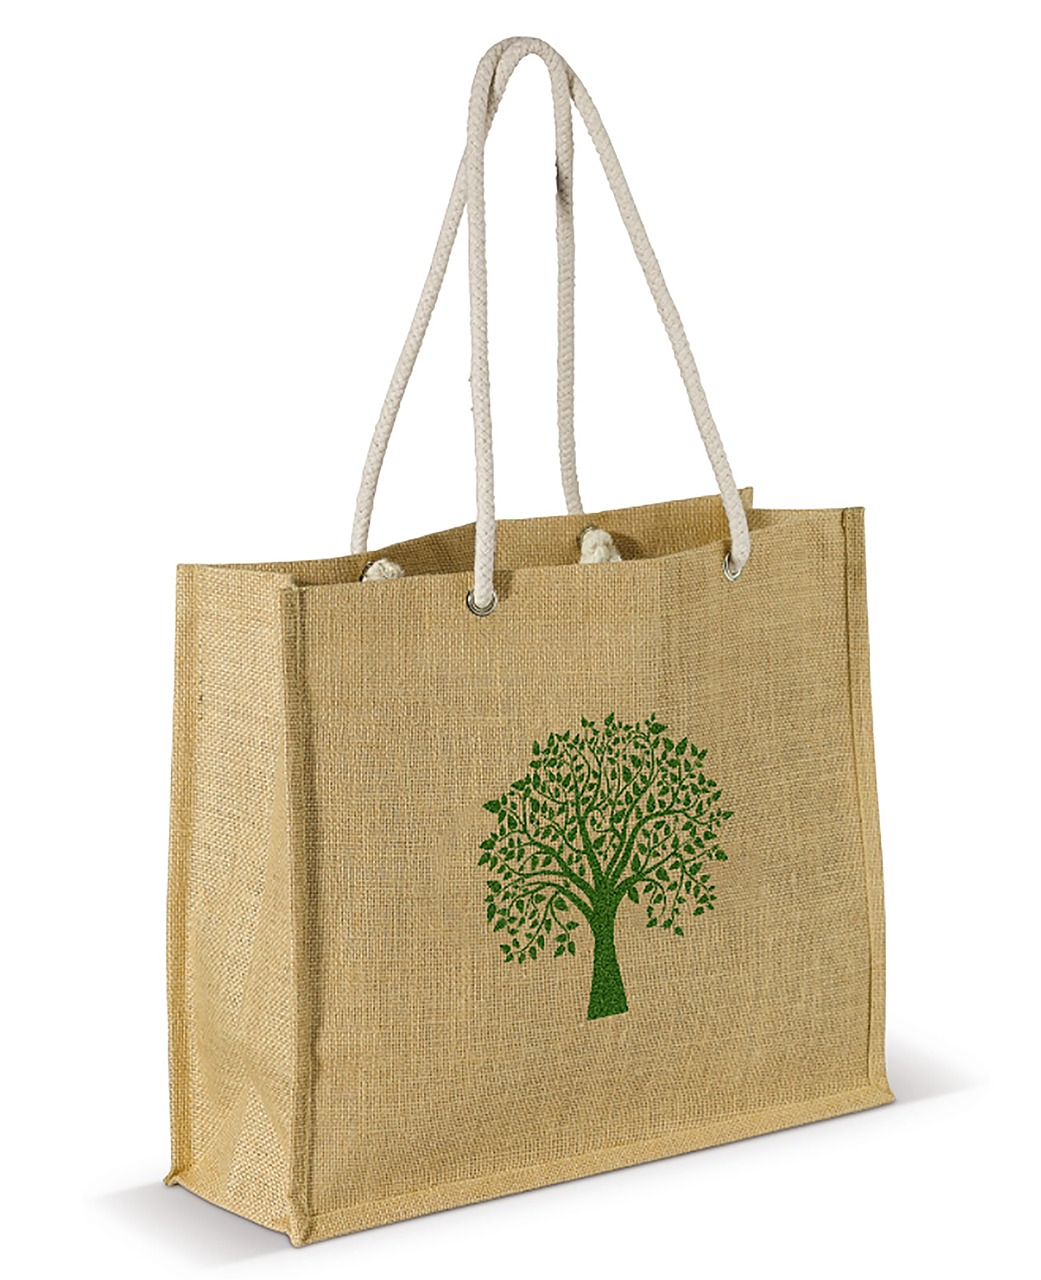
\includegraphics[width=0.9\columnwidth]{../../../FIGURES/divers/doggybag.jpg}
        \end{figure}
    \end{minipage}
\end{frame}

\end{document}
